\documentclass[a3paper, landscape, border=1cm]{standalone}

\usepackage{tikz}

\begin{document}

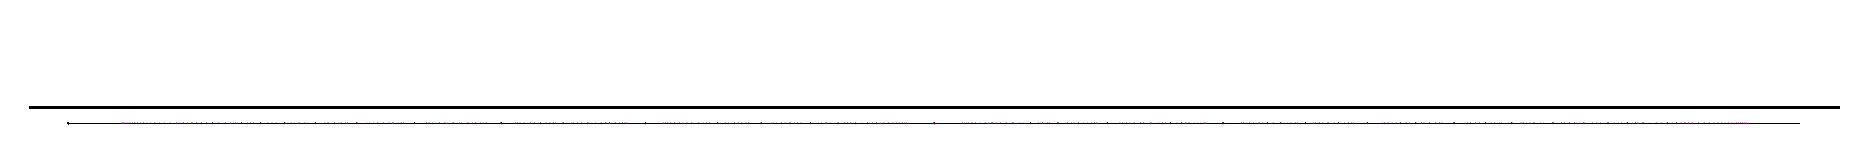
\begin{tikzpicture}

% Parametri generali
\def\length{22}           % Lunghezza della linea
% solitamente .8
\def\spacing{0}         % Distanza tra le linee
\def\numLines{32}         % Numero di linee
\def\frameMargin{0.5}     % Margine per la cornice
\def\topSpace{1}          % Spazio extra prima della cornice superiore
\def\timeLineSpace{.2}    % Spazio tra la cornice e le linee
\def\gridWidth{\length + 2*\frameMargin}  % Larghezza della griglia completa (include margini)
\def\minOpacity{0.3}      % Opacità minima alla fine della linea
\def\fixedDashLength{.8}
\def\pointRadius{.3pt}
% Ciclo per ripetere il disegno 3 volte lungo l'asse x
\foreach \k in {0} {
    % Spostamento orizzontale per ciascuna griglia
    \begin{scope}[shift={(\k*\gridWidth,0)}]

    % Cornice sopra
    \draw[thick] (-\frameMargin, -\topSpace) -- (\length+\frameMargin, -\topSpace);
    \draw[thick, opacity=0] (-\frameMargin, 0) -- (\length+\frameMargin, 0);

    % Loop per disegnare le linee
    \foreach \i in {1,...,\numLines} {
        % Coordinate della linea
        \def\y{-\i*\spacing-\topSpace-\timeLineSpace}  % La y si abbassa ogni volta, includendo lo spazio extra

 
        % Disegno della linea normale con opacità
        \draw[thick, color=black, opacity=.3, line width=.1px] (0, \y) -- (\length, \y);

        % Calcolo la divisione
        \ifnum\i>1
           \pgfmathsetmacro\division{\i-1}  % Numero di divisioni
            \foreach \j in {1,...,\division} {
                \pgfmathsetmacro\xPos{\j*\length/(\division+1)}  % Posizione del punto
                \fill[violet] (\xPos, \y) circle (\pointRadius);  % Disegno il punto con colore variabile

                % Disegna il punto con bordo e senza riempimento
               % \draw[draw=black, fill=none] (\xPos, \y) circle (\pointRadius);  % Cerchio bucato con bordo



               % Disegna la linea verticale tratteggiata passando per il punto
            %\draw[dashed,  dash pattern=on 1pt off 3pt, opacity=.6] (\xPos, -\spacing*\numLines-\spacing-\timeLineSpace-\topSpace) -- (\xPos, \y); 
            }
        \fi
    }
    % Aggiungi punti all'inizio di ogni riga
    \foreach \i in {1,...,\numLines} {
        % Coordinate del punto
        \def\y{-\i*\spacing-\topSpace-\timeLineSpace}  % La y si abbassa ogni volta, includendo lo spazio extra
        \fill[black] (0, \y) circle (\pointRadius);  % Disegna il punto all'inizio della riga

       % Disegna il punto all'inizio della riga con bordo e senza riempimento
        %\draw[draw=black, fill=none] (0, \y) circle (\pointRadius);  % Cerchio bucato con bordo
    }

    % Cornice sotto (non visibile per ora, con opacity=0)
    \draw[thick, opacity=0] (-\frameMargin, -\spacing*\numLines-\spacing-\timeLineSpace-\topSpace) -- (\length+\frameMargin,  -\spacing*\numLines-\spacing-\timeLineSpace-\topSpace);

    \end{scope}
}

\end{tikzpicture}

\end{document}
